\documentclass[tikz,border=2pt]{standalone}
\usepackage{amsmath}
\usepackage{amssymb}
\usepackage{pgfplots}
\pgfplotsset{compat=1.18}
\usetikzlibrary{arrows.meta}
\begin{document}
% Unit square V. At the corner p=(1,1): N_V(p)={a>=0}, drawn translated to p, with the supporting line x1+2x2=3 (normal (1,2)).
% At the edge point (1,1/2): N_V={(t,0): t>=0}, a single half-line.
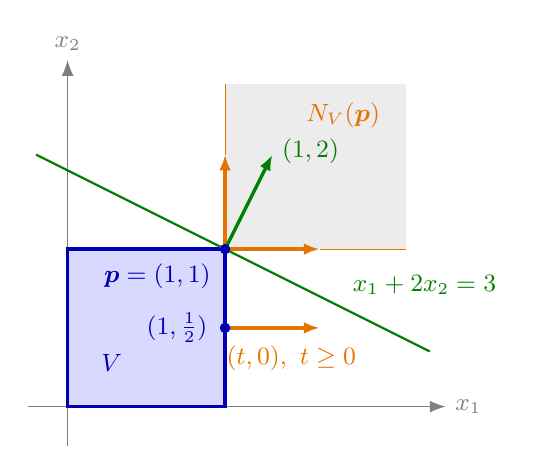
\begin{tikzpicture}[font=\small, >={Latex[length=2mm]}, x=2.0cm, y=2.0cm]
  \fill[gray!15] (1,1) -- (2.15,1) -- (2.15,2.05) -- (1,2.05) -- cycle;
  \fill[blue!15] (0,0) rectangle (1,1);
  \draw[gray, ->] (-0.25,0) -- (2.4,0) node[anchor=west] {$x_1$};
  \draw[gray, ->] (0,-0.25) -- (0,2.2) node[anchor=south] {$x_2$};
  \draw[blue!70!black, very thick] (0,0) rectangle (1,1);
  \node[blue!70!black] at (0.28,0.28) {$V$};
  % supporting line at the corner
  \draw[green!50!black, thick] (-0.2,1.6) -- (2.3,0.35);
  \node[green!50!black, anchor=south west] at (1.75,0.65) {$x_1+2x_2=3$};
  % normal cone at the corner, translated to p
  \draw[orange!90!black, very thick, ->] (1,1) -- (1.6,1);
  \draw[orange!90!black, very thick, ->] (1,1) -- (1,1.6);
  \draw[orange!90!black, thin] (1.6,1) -- (2.15,1);
  \draw[orange!90!black, thin] (1,1.6) -- (1,2.05);
  \draw[green!50!black, very thick, ->] (1,1) -- (1.3,1.6);
  \node[green!50!black, anchor=west] at (1.3,1.62) {$(1,2)$};
  \node[orange!90!black] at (1.75,1.85) {$N_V(\boldsymbol{p})$};
  \fill[blue!70!black] (1,1) circle (1.9pt);
  \node[blue!70!black, anchor=north east] at (0.97,0.97) {$\boldsymbol{p}=(1,1)$};
  % edge point
  \draw[orange!90!black, very thick, ->] (1,0.5) -- (1.6,0.5);
  \fill[blue!70!black] (1,0.5) circle (1.9pt);
  \node[blue!70!black, anchor=east] at (0.95,0.5) {$(1,\tfrac{1}{2})$};
  \node[orange!90!black, anchor=north] at (1.42,0.45) {$(t,0),\ t\geq0$};
\end{tikzpicture}
\end{document}
